\documentclass{beamer}

\definecolor{theme}{RGB}{28,90,127}
\definecolor{almostblack}{HTML}{262626}
\setbeamercolor{normal text}{fg=almostblack}

\usecolortheme[named=theme]{structure}
\usecolortheme{dolphin}  % outer color theme
\usecolortheme{orchid}  % inner color theme

% modified version of default frametitle with horizontal separation line
\makeatletter
\setbeamertemplate{frametitle}{
  \ifbeamercolorempty[bg]{frametitle}{}{\nointerlineskip}%
  \@tempdima=\textwidth%
  \advance\@tempdima by\beamer@leftmargin%
  \advance\@tempdima by\beamer@rightmargin%
  \begin{beamercolorbox}[sep=0.3cm,left,wd=\the\@tempdima]{frametitle}
    \usebeamerfont{frametitle}%
    \vbox{}\vskip-2ex%
    \if@tempswa\else\csname beamer@fteleft\endcsname\fi%
    \strut\insertframetitle\strut\par%
    {%
      \ifx\insertframesubtitle\@empty%
      \else%
      {\usebeamerfont{framesubtitle}\usebeamercolor[fg]{framesubtitle}\insertframesubtitle\strut\par}%
      \fi
    }%
    \vskip.45ex%
    \hrule %height .6pt%
    \vskip-1.45ex%
    \if@tempswa\else\vskip-.3cm\fi%
  \end{beamercolorbox}%
}
\makeatother

% clean up footer
\beamertemplatenavigationsymbolsempty
\setbeamertemplate{footline}[frame number]

\useinnertheme{default}
\setbeamertemplate{itemize item}{\raise.35ex\hbox{\vrule width .7ex height .7ex}}
\setbeamertemplate{itemize subitem}{\raise.35ex\hbox{\vrule width .6ex height .6ex}}

% for backup slides
\usepackage{appendixnumberbeamer}

\usepackage{graphicx}
\graphicspath{{fig/}}

\usepackage{amsmath}
\usepackage{amssymb}
\usepackage{tikz}

\newcommand{\avg}[1]{\langle #1 \rangle}
\newcommand{\nch}{N_\text{ch}}
\newcommand{\vnk}[2]{v_#1\{#2\}}
\newcommand{\tran}{^\intercal}
\newcommand{\trento}{T\raisebox{-.5ex}{R}ENTo}
\newcommand{\order}[1]{$\mathcal O(10^{#1})$}
\newcommand{\x}{\mathbf x}
\newcommand{\y}{\mathbf y}
\newcommand{\z}{\mathbf z}
\newcommand{\xs}{\x_\star}
\newcommand{\zs}{\z_\star}
\newcommand{\yexp}{\y_\text{exp}}
\newcommand{\zexp}{\z_\text{exp}}

\title{Quantifying properties of hot and dense QCD matter through systematic model-to-data comparison}
\author{Jonah Bernhard}
\institute{QCD group meeting}
\date{\today}


\begin{document}


\section{Title}

\begin{frame}[plain,noframenumbering]
  \maketitle
  \tiny
  J.~E.~Bernhard, P.~W.~Marcy, C.~E.~Coleman-Smith, S.~Huzurbazar, R.~L.~Wolpert, and S.~A.~Bass,
  arXiv:1502.00339 [nucl-th].
\end{frame}


\section{Introduction}

\begin{frame}{Model-to-data comparison}
  \centering
  \def\tw{\textwidth}
  \vspace{.03\tw}
  \begin{tikzpicture}[semithick]
    \def\pw{.33\tw}
    \def\dx{.55\tw}
    \def\dy{.26\tw}
    \node (lhc) {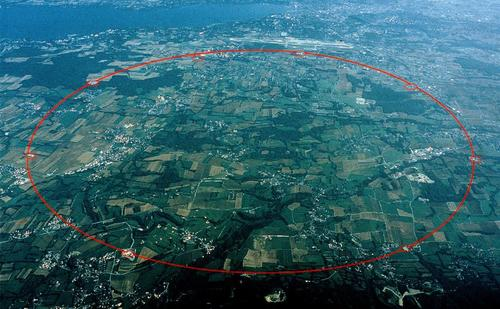
\includegraphics[width=\pw]{third_party/lhc}};
    \node[below of=lhc, node distance=\dy] (expevent)
      {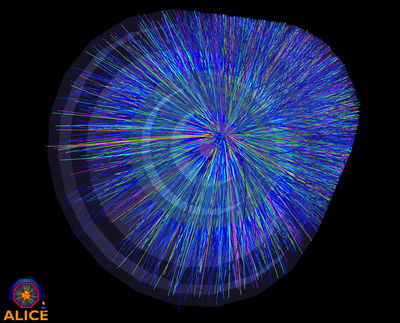
\includegraphics[width=.25\tw]{third_party/alice_event}};
    \node[below of=expevent, node distance=\dy] (expdata)
      {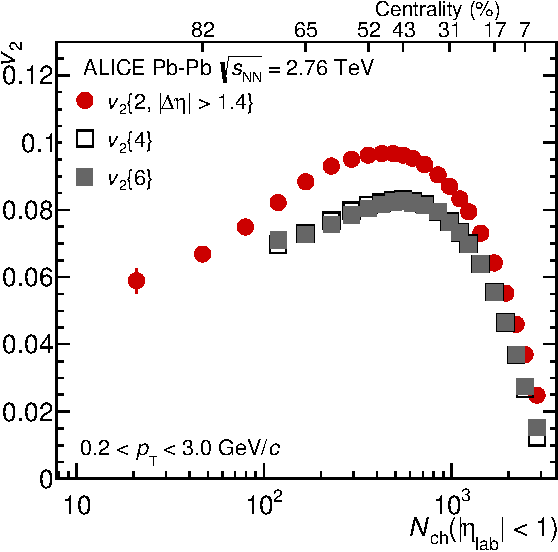
\includegraphics[width=.22\tw]{third_party/alice_data}};
    \node[right of=lhc, node distance=\dx, draw, thin,
          text width=\pw, text centered, inner sep=1ex] (modelinput)
      {\textbf{Model} \\ Initial conditions, \\ $\tau_0$, $\eta/s$, \ldots};
    \node[right of=expevent, node distance=\dx, draw, thin,
          text width=\pw, text centered, inner sep=1ex] (modelevo) {
        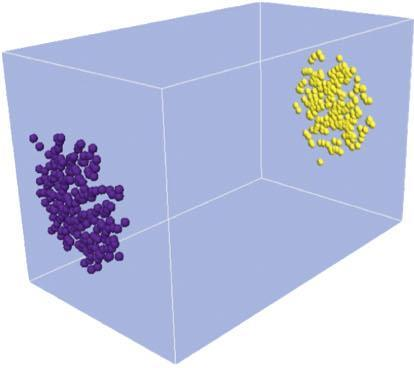
\includegraphics[width=.33\tw]{third_party/evolution1}
        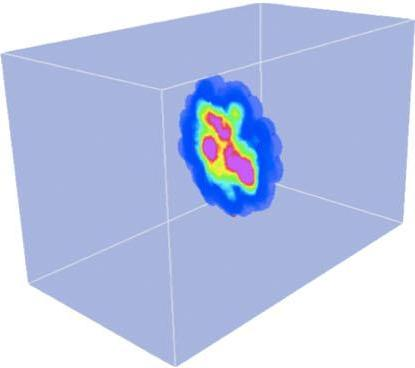
\includegraphics[width=.33\tw]{third_party/evolution2}
        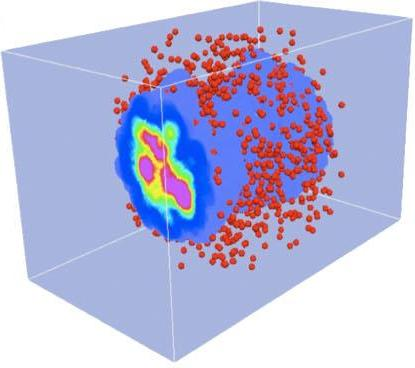
\includegraphics[width=.33\tw]{third_party/evolution3} \\
        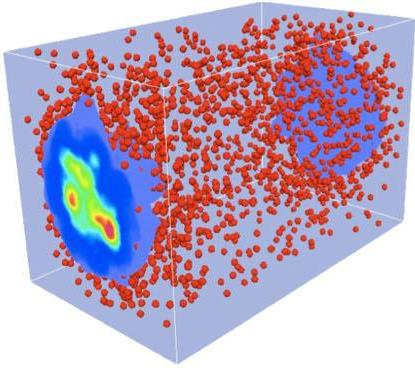
\includegraphics[width=.33\tw]{third_party/evolution4}
        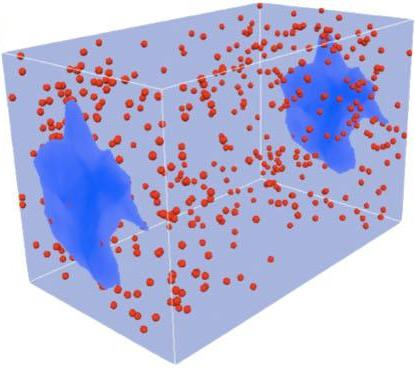
\includegraphics[width=.33\tw]{third_party/evolution5}
      };
    \node[right of=expdata, node distance=\dx, draw, thin] (modeldata)
      {\includegraphics[width=.4\tw]{prior_draws}};
    \path[->] (lhc)        edge (expevent)
              (expevent)   edge (expdata)
              (modelinput) edge (modelevo)
              (modelevo)   edge (modeldata);
    \draw[densely dashed,<->] (expdata) -- coordinate (midpt) (modeldata);
    \draw[densely dashed,->] (midpt) |- (modelinput);
  \end{tikzpicture}
\end{frame}


\begin{frame}{Measuring QGP $\eta/s$}
  \begin{enumerate}
    \item Observe experimental $v_n$
    \item Run model with variable $\eta/s$
    \item Constrain $\eta/s$ by matching $v_n$
  \end{enumerate}
  \medskip
  \centering
  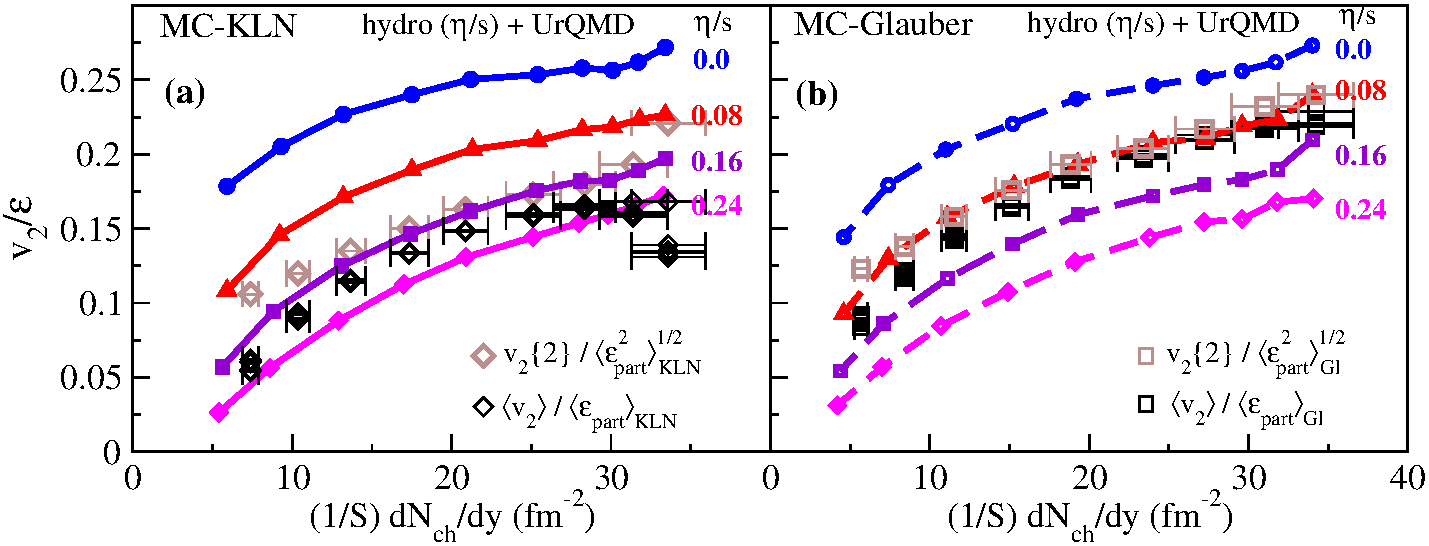
\includegraphics[width=\textwidth]{third_party/osu}
  \flushright
  \tiny
  H.~Song, S.~A.~Bass, U.~Heinz, T.~Hirano, and C.~Shen, \\
  PRL\ {\bf 106}, 192301 (2011), arXiv:1011.2783 [nucl-th].
\end{frame}


\begin{frame}{Extracting QGP properties}
  \vspace{1em}
  \begin{columns}
    \column{.45\textwidth}
    \begin{center}
      \bf Older work
    \end{center}
    \begin{itemize}
      \item Average calculations
      \item Only $\eta/s$
      \item Several discrete values
      \item Qualitative constraints lacking uncertainty
    \end{itemize}

    \column{.50\textwidth}
    \begin{center}
      \bf New projects
    \end{center}
    \begin{itemize}
      \item Event-by-event model
      \item Vary many parameters
      \item Continuous parameter space
      \item Quantitative constraints including uncertainty
    \end{itemize}
  \end{columns}

  \vspace{2em}
  \tiny
  See also, e.g.: \\
  \begin{itemize}
    \item J.~Novak, K.~Novak, S.~Pratt, C.~Coleman-Smith, and R.~Wolpert, \\
      PRC \textbf{89}, 034917 (2014), arXiv:1303.5769 [nucl-th].
    \item R.~A.~Soltz, I.~Garishvili, M.~Cheng, B.~Abelev, A.~Glenn, J.~Newby, L.~A.~Linden Levy, and S.~Pratt, \\
      PRC {\bf 87}, 044901 (2013), arXiv:1208.0897 [nucl-th].
  \end{itemize}

  \tikz[overlay,remember picture]
    \node[xshift=-3ex,yshift=4ex] at (current page.center)
    {$\color{theme}\Large\boldsymbol\longrightarrow$};
\end{frame}


\section{Method}

\begin{frame}{Strategy}
  \begin{enumerate}
    \item Choose set of salient model parameters
      \begin{itemize}
        \item physical properties
        \item model nuisance parameters
      \end{itemize}
    \item Run model at a small $\mathcal O(10^1$--$10^2)$ set of parameter points
    \item Interpolate with a Gaussian process emulator \\
      $\rightarrow$ fast surrogate to actual model
    \item Systematically explore parameter space with Markov chain Monte Carlo (MCMC)
    \item Calibrate model emulator to optimally reproduce data \\
      $\rightarrow$ extract probability distributions for each parameter
  \end{enumerate}
\end{frame}


\begin{frame}{Event-by-event model}
  \begin{itemize}
    \item MC-Glauber \& MC-KLN initial conditions \\
      \hspace{1em} {\tiny H.-J.\ Drescher and Y.\ Nara, PRC {\bf 74}, 044905 (2006).}
    \item Viscous 2+1D hydro \\
      \hspace{1em} {\tiny H.\ Song and U.\ Heinz, PRC {\bf 77}, 064901 (2008).}
    \item Cooper-Frye hypersurface sampler \\
      \hspace{1em} {\tiny C.~Shen, Z.~Qiu, H.~Song, J.~Bernhard, S.~Bass, and U.~Heinz, arXiv:1409.8164 [nucl-th].}
    \item UrQMD \\
      \hspace{1em} {\tiny S.\ Bass \emph{et.\ al.}, Prog.\ Part.\ Nucl.\ Phys.\  {\bf 41}, 255 (1998).} \\[-1ex]
      \hspace{1em} {\tiny M.\ Bleicher \emph{et.\ al.}, J.\ Phys.\ G {\bf 25}, 1859 (1999).}
  \end{itemize}
\end{frame}


\begin{frame}{Computer experiment design}
  \centering
  \includegraphics{design}
\end{frame}


\begin{frame}{Training data}
  \centering
  Model calculations for each design point \\
  \bigskip
  \includegraphics{prior_draws}
  \flushright
  \tiny
  Data points: ALICE Collaboration, Pb-Pb collisions at $\sqrt{s_\text{NN}} = 2.76$ TeV \\
  B.~B.~Abelev {\it et al.}, PRC {\bf 90}, 054901 (2014), arXiv:1406.2474 [nucl-ex].
\end{frame}


\begin{frame}{Gaussian process emulator}
  \vspace{1ex}
  \begin{itemize}
    \item Non-parametric interpolation
    \item Predicts \emph{probability distributions}
      \begin{itemize}
        \item Narrow near training points, wide in gaps
      \end{itemize}
    \item Fast ``surrogate'' to actual model
  \end{itemize}
  \medskip
  \centering
  \includegraphics{gp}
  \flushright
  \footnotesize
  \begin{tabular}{ll}
    dashed line = GP mean &
    colored lines = random samples \\
    grey band = $2\sigma$ confidence interval &
    dots = training points
  \end{tabular}
\end{frame}


\begin{frame}{Multivariate output}
  \centering
  \includegraphics{pc_var} \\
  \includegraphics{pc_scatter}
\end{frame}


\begin{frame}{Validation}
  \centering
  \includegraphics{validation}
\end{frame}


\begin{frame}{Bayes' theorem}
  \begin{equation*}
    P(\xs|X,Y,\yexp) \propto P(X,Y,\yexp|\xs) P(\xs)
  \end{equation*}
  \begin{itemize}
    \item $P(\xs)$ = prior \\
      $\rightarrow$ initial knowledge of $\xs$
    \item $P(X,Y,\yexp|\xs)$ = likelihood \\
      $\rightarrow$ prob.\ of observing $(X, Y, \yexp)$ given proposed $\xs$
    \item $P(\xs|X,Y,\yexp)$ = posterior \\
      $\rightarrow$ prob.\ of $\xs$ given observations $(X, Y, \yexp)$
  \end{itemize}
\end{frame}


\section{Results}

\begin{frame}[plain,noframenumbering]
  \centering
  \LARGE
  Posterior distributions
\end{frame}


\begin{frame}{}
  \vspace{1ex}
  \centering
  \includegraphics{cal_post_glb}
  \tikz[remember picture, overlay]
    \node[color=gray, rotate=45, yshift=-3em] at (current page.north west)
    {Glauber};
\end{frame}


\begin{frame}{}
  \vspace{1ex}
  \centering
  \includegraphics{cal_post_kln}
  \tikz[remember picture, overlay]
    \node[color=gray, rotate=45, yshift=-3em] at (current page.north west)
    {KLN};
\end{frame}


\begin{frame}{Posterior samples}
  \centering
  \only<1>{
    Model calculations over full design space \\[4ex]
    \includegraphics{prior_draws}
  }
  \only<2>{
    Emulator predictions from calibrated posterior \\[4ex]
    \includegraphics{post_draws}
  }
\end{frame}


\begin{frame}{$\eta/s$ posteriors}
  \begin{itemize}
    \item
      \parbox{3.5em}{Glauber}
      \parbox{5em}{$\eta/s \sim 0.06$,}
      95\% C.I.\ $\sim$ 0.02--0.10
    \item
      \parbox{3.5em}{KLN}
      \parbox{5em}{$\eta/s \sim 0.16$,}
      95\% C.I.\ $\sim$ 0.12--0.21
  \end{itemize}
  \medskip
  \centering
  \includegraphics{post_compare}
\end{frame}


\section{Conclusion}

\begin{frame}{Summary \& outlook}

\end{frame}


\appendix


\begin{frame}{Training the emulator}
  Covariance function:
  \begin{equation*}
    \sigma(x, x') = \exp\biggl( -\frac{|x - x'|^2}{2\ell^2} \biggr) +
                    \sigma_n^2\delta_{xx'}
  \end{equation*}
  $(\ell, \sigma_n)$ are unknown hyperparameters \\
  \bigskip
  \centering
  \includegraphics{training}
\end{frame}


\end{document}
